\chapter{Frontend}
\section{Auswahl einer Physics-Engine}

\begin{quote}
	\href{https://github.com/Transport-Protocol/MBC-Ping-Pong/issues/3}{Auswahl einer geeigneten 2D-/Physiksengine \#3}
	\newline
	Die Darstellung auf dem Anzeigegerät ist über den DOM nicht möglich, da die Bewegung des Balls und der Schläger zu schnell werden. Zudem wird auch die Physik auf dem Anzeigegeräts berechnet. Hierfür ist eine Kollisionserkennung erforderlich.
\end{quote}
Für die physikalisch korrekte Kollision des Balles mit der Spielwelt und den Schlägern haben wir uns entschieden eine Physics-Engine zu verwenden.

\subsection{Matter.JS}
Matter js ist eine sehr mächtige Engine. Sie unterstützt viele Formen und Physikalische Eigenschaften wie zum Beispiel Masse und wirkende Kräfte auf die jeweiligen Objekte. 
Es besteht die Möglichkeit physikalische Objekte zusammen zusetzen und sogar diese Elastisch erscheinen zu lassen, so ist es beispielsweise möglich Stoff oder schwingende Seile zu erstellen.
Nach mehrstündiger Einarbeitung kam ich zu dem Schluss das diese Engine für unser Projekt nicht geeignet ist.
Gründe hierfür sind:
\begin{itemize}
	\item
	      Zu Komplex:
	      Die Einrichtung des Spielfeldes erwies sich als überaus schwierig. Gute Anleitungen für einfache Szenarien fehlten, die verfügbaren Anleitungen sind zu grundlegend beschrieben.
	      Ebenfalls half die Anleitung der Engine nicht bei der Verwendung der einzelnen Komponenten.
	\item
	      Die Positionierung der Objekte bezog sich immer auf den Mittelpunkt des Objektes, man kann beispielsweise kein Rechteck von (x,y) nach (x1,y1) erstellen sondern muss den Mittelpunkt und die Abmaße des Objektes angeben.
	\item
	      Physik nicht immer korrekt. Die Engine sollte den Ball richtig von einer Ebene abprallen lassen, diese Engine allerdings lies den Ball teilweise an Plattformen abrollen obwohl keine Schwerkraft vorhanden war. Ich schließe darauf das die Engine Reibungskräfte und vielleicht sogar Anziehungskräfte zwischen den Objekten herstellt. Für unser Projekt ist dies aber nicht zu gebrauchen.
	\item
	      Schwer zu debuggen. Während meiner Versuche bin ich immer wieder auf Probleme gestoßen. Einige der Debugausgaben ließen sich gut ableiten und waren hilfreich. 
	      Allerdings bin ich auch auf einige Probleme gestoßen welche nicht in den Debugausgaben behandelt wurde. Meine letzten Versuche endeten alle darin das der Browser gecrasht ist aufgrund eines Memory-leaks.
\end{itemize}
\subsection{Phaser.io}
Phaser.io beschreibt sich selber als html5 Game Framework. Es wurde nach dem mobile-first Prinzip entwickelt und ist opensource.
Die Entwicklung des gewünschten Prototypen erwies sich als sehr leicht, da es viele gute Beispiele gibt.
Die Engine unterstützt von Haus aus eine Arcade-Physic, diese ist perfekt für unser Projekt. Sie beinhaltet Kollisions und Bewegungsfunktionen für den 2-Dimensionalen Raum
\subsection{Erstellung eines Prototypen}
In Phaser erstellt man ein Spiel über den Aufruf 'new Phaser.Game(...) die ersten Beiden Argumente geben die Dimensionen des Spielfeldes an, also die Weite und Höhe in Pixeln. 
\newline
Der Nächste Parameter bestimmt die Render-Engine. 
Mögliche Werte sind 'Phaser.CANVAS', 'Phaser.WEBGL' oder 'Phaser.AUTO', wenn 'Phaser.AUTO' verwendet wird so probiert die Engine erst WebGL aus und für den Fall das der Browser WebGL nicht unterstützt wird Canvas verwendet.
\newline
Das nächste Argument gibt das Ziel im DOM an, wenn man diesen Parameter nicht setzt wird das Spiel einfach im Body angehängt.
\newline
Man kann als 5. Argument ein Startzustand angeben. Zustände kann man sich wie Spielszenen vorstellen. 
Ich habe mich dafür entschieden die Spielszene erst später hinzuzufügen, das bietet mir den Vorteil das ich diesem Zustand einen Namen geben kann und diesen Später erneut verwenden könnte.
\newpage
Eine Szene bzw. einen Spielzustand kann man per game.state.add('name',State) vobei 'game' die Instanz des Spiels darstellt.
Gestartet wird der Zustand per: 'game.state.start('name)'
Ein Zustand ist wie folgt aufgebaut:
\begin{lstlisting}
{
    preload: function () {
 
    },
 
    create: function () {
 
    },
 
    update: function () {
 
    },
};
\end{lstlisting}
Zu den einzelnen Funktionen:
\begin{itemize}
	\item
	      \textbf{preload:} Diese Funktion ist für das Vorladen von Assets gedacht. Beispielsweise Sprites oder Sounds werden hier vorgeladen damit während das Spiel läuft ohne Ladezeit zur Verfügung stehen.
	\item
	      \textbf{create:} Hier werden alle Objekte erstellt die mit dem Beginn des Spielzustandes vorhanden sein sollen. Hier kann man auch Starteigenschafen wie Geschwindigkeit, Schwerkraft oder Ausrichtung setzen.
	\item
	      \textbf{update:} Die update Funktion wird für die Berechnung jedes Frames aufgerufen. In dieser Funktion werden beispielsweise Kollisionen überprüft und darauf reagiert.
\end{itemize}
\newpage
Für den Ball des Ping Pong Prototypen habe ich diese Funktionen wie folgt erstellt:
\begin{itemize}
	\item
	      \textbf{preload:}
	      \newline
	      Laden des Sprites in den Namen 'ball':
	      \newline
	      \begin{lstlisting}
game.load.image('ball','assets/testBall.png');
	      \end{lstlisting}
	      Bekanntmachung der Ball Variable: this.ball
	\item
	      \textbf{create:}
	      \newline Erstellen des Balls und einstellen des Ausrichtungspunktes in die Mitte des Sprites:
	      \begin{lstlisting}
this.ball = 
 game.add.sprite(game.world.centerX, game.world.centerY, 'ball');
this.ball.anchor.set(0.5, 0.5);
	      \end{lstlisting}
	      Aktivieren der Physik für den Ball:
	      \begin{lstlisting}
game.physics.startSystem(Phaser.Physics.ARCADE);
game.physics.enable(this.ball, Phaser.Physics.ARCADE);
	      \end{lstlisting}
	      Als nächstes hab ich den Ball so konfiguriert das er mit den Spielfeldrändern kollidiert:
	      \begin{lstlisting}
this.ball.checkWorldBounds = true;
this.ball.body.collideWorldBounds = true;
	      \end{lstlisting}
	      Damit der Ball keine zusätzliche Geschwindigkeit beim Kollidieren mit einem anderem sich bewegendem Objekt erhält habe ich ihn 'unbeweglich' gemacht, damit erhält der Ball keine zusätzlichen Impulse von anderen Objekten.
	      \begin{lstlisting}
this.ball.body.immovable = true; 
	      \end{lstlisting}
	      Und das er keine Geschwindigkeit verliert beim Abprallen:
	      \begin{lstlisting}
this.ball.body.bounce.set(1);
	      \end{lstlisting}
	      Als letztes musste ich dem Ball nur noch einen Startimpuls geben:
	      \begin{lstlisting}
this.ball.body.velocity.setTo(200,0);
	      \end{lstlisting}
	\item
	      \textbf{update:} 
	      \newline Eine Update Funktion war nicht notwendig da der Ball im Prototypen nur mit dem Spielfeld kollidieren soll.
	      Für die späteren Versionen muss hier die Kollision mit den Schlägern und anderen Objekten definiert werden.
\end{itemize}
\newpage
Der fertige Prototyp sieht so aus:
\begin{figure}[ht]
	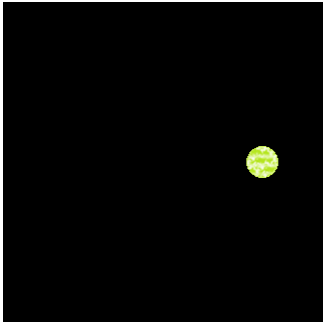
\includegraphics[scale=1]{frontend/prototype-0.png}
	\centering
	\caption{Erster Prototyp}
	\label{figx}
\end{figure}
\newpage
\section{Analyse - Steuerung}
\begin{quote}
	\href{https://github.com/Transport-Protocol/MBC-Ping-Pong/issues/11}{Analyse - Steuerung \#11}
	\newline
	\textit{Die Steuerung des Spiels erfolgt über das Handydisplay. Jedes Handy ist unterschiedlich groß, zudem sollte der Schläger nicht springen können.}
\end{quote}
Es zu analysieren wie sich verschiedene Auflösungen und verschiedene Pixeldichten auf das Spielgefühl auswirken können.
Denkbar ist das Geräte mit einer geringen Pixeldichte gegenüber Spielern mit einer hohen Pixeldichte im Vorteil sind da aus Geräten mit einer hohen Pixeldichte sehr viel kleinere Gesten zur Steuerung ausreichen.
\newline
\textbf{Zielsetzung dieser Analyse}
\begin{enumerate}
	\item
	      \textbf{Feststellung} Es soll festgestellt werden in wie weit sich ein Unterschied der Pixeldichte auf die Spielweise auswirken kann.
	\item
	      \textbf{Behandlung} Es soll geprüft werden ob sich eine mögliche Unfairness beheben lässt und ein mögliches Konzept erstellt werden.
\end{enumerate}
\subsection{Feststellung der Auswirkung verschiedener Pixeldichten}
\subsection{Behandeln verschiedener Pixeldichten}
\paragraph{Ermitteln von der PPI im Browser} Es wird nach vorhanden Lösungen zum erkennen der Pixeldichte in PPI bzw DPI gesucht.
Die gefundenen Beispiele werden dann mit verschiedenen Geräten getestet und die Ergebnisse mit den tatsächlichen DPI verglichen.
\newline\textbf{Die Testgeräte}
\begin{enumerate}
	\item \begin{tabular}{cc}
	      Name & PC Monitor\\
	      Diagonale & 23.6zoll\\
	      Auflösung & 1920*1080\\
	      Pixeldichte & 93 PPI \\
	\end{tabular}
	\item \begin{tabular}{cc}
	      Name & Samsung Galaxy S4\\
	      Diagonale & 4.99zoll\\
	      Auflösung & 1920*1080\\
	      Pixeldichte & 441 PPI
	\end{tabular}
	\item \begin{tabular}{cc}
	      Name & Samsung Galaxy Tab A\\
	      Diagonale & 9.7zoll\\
	      Auflösung & 1024*768\\
	      Pixeldichte & 132 PPI\\
	\end{tabular}
\end{enumerate}
\begin{itemize}
	\item
	      \textbf{http://www.infobyip.com/detectmonitordpi.php} Eine Website zur Ermittlung der DPI. Es wird ein Quadrat per CSS auf eine bestimmte Größe, zum Beispiel 1 Zoll, formatiert und dann die Größe in Pixeln ausgelesen. Auf diese Weise lässt sich ein DPI wert berechnen.
	      \newline
	      Tests:
	      \begin{enumerate}
	      	\begin{tabular}{ccc}
	      		                     & Erwarteter Wert & Ermittelter Wert           \\
	      		PC Monitor 1         &                 &                            \\
	      		Pixeldichte          & 93 DPI          & \colorbox{red!30}{96 DPI}  \\
	      		Größe des Feldes     & 8 cm            & \colorbox{red!30}{8.2 cm}  \\
	      		                     &                 &                            \\
	      		Samsung Galaxy S4    &                 &                            \\
	      		Pixeldichte          & 441 DPI         & \colorbox{red!30}{288 DPI} \\
	      		Größe des Feldes     & 8 cm            & \colorbox{red!30}{1.8 cm}  \\
	      		                     &                 &                            \\
	      		Samsung Galaxy Tab A &                 &                            \\
	      		Pixeldichte          & 132 DPI         & \colorbox{red!30}{96 DPI}  \\
	      		Größe des Feldes     & 8 cm            & \colorbox{red!30}{5.7cm}   \\
	      	\end{tabular}
	      \end{enumerate}
	      Getestet wurde jeweils mit Firefox & Chrome, der PC Monitor wurde auch noch mit dem Edge Browser getestet. Die Ergebnisse waren allesamt für das Gerät identisch.
	      \newline
	      \textbf{Ergebnis:} Die DPI wurden nicht korrekt erkannt. Die Werte weichen auf dem Mobiltelefon um \underline{77.5\%} ab.
\end{itemize}
\newpage
\paragraph{Verwenden von 'window.devicePixelRatio'} Die Eigenschaft \textit{window.devicePixelRatio} gibt das Verhältnis der Größe der physikalischen Pixel des aktuellen Displays zu der Größe der Geräteunabhängigen-Pixel (\textit{device independent pixels(dips)}) wieder.
\begin{displaymath}
	window.devicePixelRatio = physical pixels / dips 
\end{displaymath}

Es wird vor allem dafür genutzt um eine Einheitliche Darstellung von Webinhalten auf verschiedenen Displaygrößen zu erreichen.
\newline
Die Methode klingt sehr vielversprechend, also entschied ich einen Test zu erstellen. Meine Idee ist es ein Quadrat zeichnen zu lassen bei dem die Größe abhängig von dem devicePixelRatio ist und dann die Seitenlänge auf dem Display zu messen.
Mein verwendeter Code:
\begin{lstlisting}
var c=document.getElementById("myCanvas");
var ctx=c.getContext("2d");
var w = 100*window.devicePixelRatio;
ctx.rect(20,20,w,w);
ctx.fillText(w,30,30); 
ctx.stroke(); 
\end{lstlisting}

\textbf{Tests:}
\newline
\begin{tabular}{ccc}
	Gerät                 & DevicePixelRatio & Größe TestQuadrat \\
	PC Monitor 23.6"       & 1.0              & 2.7 cm              \\
	Samsung Galaxy S4      & 3.0              & 1.9 cm              \\
	Samsung Galaxy Tab A   & 1.0              & 1.5 cm              \\
	Samsung Galaxy S3 Neo  & 2.0              & 1.3 cm              \\
	Samsung Galaxy S5 mini & 2.0              & 1.1 cm              \\
	Samsung Galaxy S7 edge & 4.0              & >4 cm               \\
\end{tabular}
\paragraph{Ergebnis:} Das Ergebnis der Tests ist leider ernüchternd. Die ersten Geräte zeigten das Quardrat allesamt in einer ähnlichen Größe. Doch auf weiteren Testgeräten zeigte sich das die Größe sehr stark variierte. Auf dem Samsung Galaxy S7 edge war das Quadrat sogar sehr viel größer als der vordefinierte Bereich.
\newpage
\subsection{Ergebis der Analyse}
Es gibt leider keine Möglichkeit eine Webapp mit exakten physikalischen Größen zu gestalten.
\paragraph{Gestaltung per CSS Einheiten} In CSS besteht die Möglichkeit Größen in CM oder Zoll zu definieren. Leider entsprechen die Werte auf Mobilen Endgeräten nicht den gewünschten Werten.
\paragraph{Gestaltung mit Device Pixel Ratio} Die Gestaltung per devicePixelRatio erscheint wesentlich genauer als die Gestaltung mit CSS Längenangaben allerdings ist auch diese Lösung sehr ungenau und lässt sich nicht einheitlich nutzen. 